%%%%%%%%%%%%%%%%%%%%%%%%%%%%%%%%%%%%%%%%%%%%%%%%%%%%%%%%%%%%
% 3.13 COMPUTATIONAL GEOMETRY
% The Composition of Advanced Mathematics
%%%%%%%%%%%%%%%%%%%%%%%%%%%%%%%%%%%%%%%%%%%%%%%%%%%%%%%%%%%%

\section{Computational Geometry}
\label{sec:computational-geometry}

\prerequisite{
Analytic Geometry, Vector Geometry, Convex Geometry,
Discrete Geometry, basic Linear Algebra, elementary
Algorithms, and basic Combinatorics.
}

\learningobjectives{
By the end of this section, the reader should be able to:
\begin{itemize}
    \item explain the purpose and scope of computational geometry;
    \item represent geometric objects numerically;
    \item use orientation tests based on determinants and cross products;
    \item test whether line segments intersect;
    \item distinguish geometric predicates from geometric constructions;
    \item formulate the planar convex hull problem;
    \item explain the main ideas of Graham scan and monotone chain algorithms;
    \item describe the gift-wrapping method;
    \item construct and interpret Voronoi diagrams;
    \item explain the dual relationship between Voronoi diagrams and Delaunay triangulations;
    \item use the empty circumcircle criterion for Delaunay triangles;
    \item formulate nearest-neighbor and closest-pair problems;
    \item explain divide-and-conquer approaches to geometric problems;
    \item describe point-in-polygon tests;
    \item explain polygon triangulation;
    \item describe sweep-line algorithms;
    \item formulate orthogonal range-searching problems;
    \item explain spatial data structures such as \(k\)-d trees and quadtrees;
    \item distinguish exact geometric reasoning from floating-point computation;
    \item explain degeneracy and general-position assumptions;
    \item recognize applications in graphics, robotics, GIS, optimization,
    scientific computing, and data analysis.
\end{itemize}
}

%%%%%%%%%%%%%%%%%%%%%%%%%%%%%%%%%%%%%%%%%%%%%%%%%%%%%%%%%%%%
\subsection{What Is Computational Geometry?}
\label{subsec:what-is-computational-geometry}
%%%%%%%%%%%%%%%%%%%%%%%%%%%%%%%%%%%%%%%%%%%%%%%%%%%%%%%%%%%%

Computational geometry studies algorithms for solving geometric problems.

The input typically consists of objects such as

\[
\boxed{
\text{points},
\quad
\text{segments},
\quad
\text{polygons},
\quad
\text{circles},
\quad
\text{polyhedra},
\quad
\text{meshes}.
}
\]

The goal is not merely to prove that a geometric object exists, but to
determine how it can be computed efficiently.

\begin{conceptbox}
Classical geometry asks:

\[
\text{What geometric relationships are true?}
\]

Computational geometry additionally asks:

\[
\boxed{
\text{How can those relationships be computed efficiently and reliably?}
}
\]
\end{conceptbox}

%%%%%%%%%%%%%%%%%%%%%%%%%%%%%%%%%%%%%%%%%%%%%%%%%%%%%%%%%%%%
\subsection{Geometry as Data}
\label{subsec:geometry-as-data}
%%%%%%%%%%%%%%%%%%%%%%%%%%%%%%%%%%%%%%%%%%%%%%%%%%%%%%%%%%%%

A point in the plane can be stored as an ordered pair

\[
p=(x,y).
\]

A segment can be represented by its endpoints

\[
\overline{pq}.
\]

A polygon can be represented by an ordered sequence of vertices

\[
\boxed{
P=(p_1,p_2,\ldots,p_n).
}
\]

Thus geometric objects become data structures that algorithms can manipulate.

%%%%%%%%%%%%%%%%%%%%%%%%%%%%%%%%%%%%%%%%%%%%%%%%%%%%%%%%%%%%
\subsection{Geometric Predicates}
\label{subsec:geometric-predicates}
%%%%%%%%%%%%%%%%%%%%%%%%%%%%%%%%%%%%%%%%%%%%%%%%%%%%%%%%%%%%

Many geometric algorithms depend on simple yes-or-no questions.

These are called \emph{geometric predicates}.

Examples include:

\[
\boxed{
\text{Is a point left of a directed line?}
}
\]

\[
\boxed{
\text{Do two segments intersect?}
}
\]

\[
\boxed{
\text{Is a point inside a circle?}
}
\]

\[
\boxed{
\text{Is a point inside a polygon?}
}
\]

Reliable predicates form the foundation of robust computational geometry.

%%%%%%%%%%%%%%%%%%%%%%%%%%%%%%%%%%%%%%%%%%%%%%%%%%%%%%%%%%%%
\subsection{Orientation of Three Points}
\label{subsec:orientation-three-points}
%%%%%%%%%%%%%%%%%%%%%%%%%%%%%%%%%%%%%%%%%%%%%%%%%%%%%%%%%%%%

Let

\[
p=(p_x,p_y),
\qquad
q=(q_x,q_y),
\qquad
r=(r_x,r_y).
\]

Define the orientation determinant

\[
\boxed{
\operatorname{orient}(p,q,r)
=
\begin{vmatrix}
q_x-p_x & q_y-p_y\\
r_x-p_x & r_y-p_y
\end{vmatrix}.
}
\]

Expanding,

\[
\boxed{
\operatorname{orient}(p,q,r)
=
(q_x-p_x)(r_y-p_y)
-
(q_y-p_y)(r_x-p_x).
}
\]

%%%%%%%%%%%%%%%%%%%%%%%%%%%%%%%%%%%%%%%%%%%%%%%%%%%%%%%%%%%%
\subsection{Interpreting the Orientation Test}
\label{subsec:orientation-interpretation}
%%%%%%%%%%%%%%%%%%%%%%%%%%%%%%%%%%%%%%%%%%%%%%%%%%%%%%%%%%%%

The sign of

\[
\operatorname{orient}(p,q,r)
\]

determines the orientation of the three points.

If

\[
\boxed{
\operatorname{orient}(p,q,r)>0,
}
\]

then \(p,q,r\) make a counterclockwise turn.

If

\[
\boxed{
\operatorname{orient}(p,q,r)<0,
}
\]

then they make a clockwise turn.

If

\[
\boxed{
\operatorname{orient}(p,q,r)=0,
}
\]

then the points are collinear.

\begin{centereddiagram}
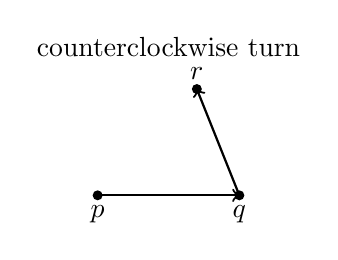
\begin{tikzpicture}[scale=.9]

\coordinate (P) at (0,0);
\coordinate (Q) at (2,0);
\coordinate (R) at (1.4,1.5);

\draw[->,thick] (P)--(Q);
\draw[->,thick] (Q)--(R);

\fill (P) circle (2pt) node[below] {$p$};
\fill (Q) circle (2pt) node[below] {$q$};
\fill (R) circle (2pt) node[above] {$r$};

\node at (1,2.1) {counterclockwise turn};

\end{tikzpicture}
\end{centereddiagram}

%%%%%%%%%%%%%%%%%%%%%%%%%%%%%%%%%%%%%%%%%%%%%%%%%%%%%%%%%%%%
\subsection{Orientation and Signed Area}
\label{subsec:orientation-signed-area}
%%%%%%%%%%%%%%%%%%%%%%%%%%%%%%%%%%%%%%%%%%%%%%%%%%%%%%%%%%%%

The orientation determinant is twice the signed area of the triangle formed
by \(p,q,r\).

Thus

\[
\boxed{
A_{\text{signed}}
=
\frac12
\operatorname{orient}(p,q,r).
}
\]

The ordinary area is

\[
\boxed{
A
=
\frac12
\left|
\operatorname{orient}(p,q,r)
\right|.
}
\]

This illustrates an important computational principle:

\begin{conceptbox}
A single determinant can encode several geometric properties at once:
orientation, collinearity, and triangle area.
\end{conceptbox}

%%%%%%%%%%%%%%%%%%%%%%%%%%%%%%%%%%%%%%%%%%%%%%%%%%%%%%%%%%%%
\subsection{Worked Example: Orientation}
\label{subsec:worked-orientation}
%%%%%%%%%%%%%%%%%%%%%%%%%%%%%%%%%%%%%%%%%%%%%%%%%%%%%%%%%%%%

\begin{workedexamplebox}{Determine the Orientation of Three Points}

Let

\[
p=(1,1),
\qquad
q=(4,2),
\qquad
r=(2,5).
\]

Compute

\[
\operatorname{orient}(p,q,r)
=
(4-1)(5-1)-(2-1)(2-1).
\]

Therefore

\[
\operatorname{orient}(p,q,r)
=
3(4)-1(1)
=
11.
\]

Since

\[
11>0,
\]

the points form a counterclockwise turn.

\begin{answerbox}
\[
\boxed{
\operatorname{orient}(p,q,r)=11>0
}
\]

so the orientation is counterclockwise.
\end{answerbox}
\end{workedexamplebox}

%%%%%%%%%%%%%%%%%%%%%%%%%%%%%%%%%%%%%%%%%%%%%%%%%%%%%%%%%%%%
\subsection{Segment Intersection}
\label{subsec:segment-intersection}
%%%%%%%%%%%%%%%%%%%%%%%%%%%%%%%%%%%%%%%%%%%%%%%%%%%%%%%%%%%%

Consider two closed line segments

\[
\overline{p_1p_2}
\]

and

\[
\overline{q_1q_2}.
\]

In the nondegenerate case, they properly intersect when the endpoints of
each segment lie on opposite sides of the line containing the other segment.

Using orientation predicates, this can be tested through

\[
\operatorname{orient}(p_1,p_2,q_1)
\]

and

\[
\operatorname{orient}(p_1,p_2,q_2),
\]

together with the corresponding orientations of \(p_1,p_2\) relative to
the line through \(q_1,q_2\).

%%%%%%%%%%%%%%%%%%%%%%%%%%%%%%%%%%%%%%%%%%%%%%%%%%%%%%%%%%%%
\subsection{Proper Segment Intersection Test}
\label{subsec:proper-segment-intersection}
%%%%%%%%%%%%%%%%%%%%%%%%%%%%%%%%%%%%%%%%%%%%%%%%%%%%%%%%%%%%

For segments in general position, a proper intersection occurs when

\[
\boxed{
\operatorname{orient}(p_1,p_2,q_1)
\operatorname{orient}(p_1,p_2,q_2)<0
}
\]

and

\[
\boxed{
\operatorname{orient}(q_1,q_2,p_1)
\operatorname{orient}(q_1,q_2,p_2)<0.
}
\]

Collinear and endpoint-touching cases must be handled separately.

%%%%%%%%%%%%%%%%%%%%%%%%%%%%%%%%%%%%%%%%%%%%%%%%%%%%%%%%%%%%
\subsection{Bounding-Box Test}
\label{subsec:bounding-box-test}
%%%%%%%%%%%%%%%%%%%%%%%%%%%%%%%%%%%%%%%%%%%%%%%%%%%%%%%%%%%%

Before performing more expensive geometric tests, algorithms often compare
axis-aligned bounding boxes.

Two segments cannot intersect if their \(x\)-coordinate intervals are
disjoint or their \(y\)-coordinate intervals are disjoint.

This inexpensive rejection test illustrates a common algorithmic strategy:

\[
\boxed{
\text{eliminate impossible cases quickly before detailed computation}.
}
\]

%%%%%%%%%%%%%%%%%%%%%%%%%%%%%%%%%%%%%%%%%%%%%%%%%%%%%%%%%%%%
\subsection{Distance Computations}
\label{subsec:computational-distance}
%%%%%%%%%%%%%%%%%%%%%%%%%%%%%%%%%%%%%%%%%%%%%%%%%%%%%%%%%%%%

For points

\[
p=(p_x,p_y),
\qquad
q=(q_x,q_y),
\]

the Euclidean distance is

\[
\boxed{
d(p,q)
=
\sqrt{
(p_x-q_x)^2+(p_y-q_y)^2
}.
}
\]

When only comparing distances, the square root is unnecessary.

Instead compare

\[
\boxed{
d^2(p,q)
=
(p_x-q_x)^2+(p_y-q_y)^2.
}
\]

This avoids an unnecessary square-root computation.

%%%%%%%%%%%%%%%%%%%%%%%%%%%%%%%%%%%%%%%%%%%%%%%%%%%%%%%%%%%%
\subsection{The Closest-Pair Problem}
\label{subsec:closest-pair-problem}
%%%%%%%%%%%%%%%%%%%%%%%%%%%%%%%%%%%%%%%%%%%%%%%%%%%%%%%%%%%%

Given

\[
P=\{p_1,\ldots,p_n\},
\]

the \emph{closest-pair problem} asks for distinct points \(p_i,p_j\) that
minimize

\[
\boxed{
\|p_i-p_j\|.
}
\]

A brute-force algorithm checks every pair.

There are

\[
\binom{n}{2}
=
\frac{n(n-1)}{2}
\]

pairs, giving quadratic running time:

\[
\boxed{
O(n^2).
}
\]

%%%%%%%%%%%%%%%%%%%%%%%%%%%%%%%%%%%%%%%%%%%%%%%%%%%%%%%%%%%%
\subsection{Divide and Conquer}
\label{subsec:closest-pair-divide-conquer}
%%%%%%%%%%%%%%%%%%%%%%%%%%%%%%%%%%%%%%%%%%%%%%%%%%%%%%%%%%%%

The planar closest-pair problem can be solved more efficiently using
divide and conquer.

The broad strategy is:

\begin{enumerate}
    \item sort the points;
    \item divide them into left and right subsets;
    \item recursively find the closest pair in each subset;
    \item inspect only a narrow strip near the dividing line;
    \item combine the results.
\end{enumerate}

This yields an algorithm with running time

\[
\boxed{
O(n\log n).
}
\]

%%%%%%%%%%%%%%%%%%%%%%%%%%%%%%%%%%%%%%%%%%%%%%%%%%%%%%%%%%%%
\subsection{Algorithmic Complexity}
\label{subsec:geometry-algorithmic-complexity}
%%%%%%%%%%%%%%%%%%%%%%%%%%%%%%%%%%%%%%%%%%%%%%%%%%%%%%%%%%%%

Computational geometry evaluates not only whether an algorithm is correct
but also how efficiently it uses resources.

Common running-time classes include

\[
\boxed{O(1)}
\]

for constant time,

\[
\boxed{O(\log n)}
\]

for logarithmic time,

\[
\boxed{O(n)}
\]

for linear time,

\[
\boxed{O(n\log n)}
\]

for near-linear sorting-type complexity, and

\[
\boxed{O(n^2)}
\]

for quadratic time.

The notation \(O(\cdot)\), read ``big O,'' describes asymptotic upper
bounds.

%%%%%%%%%%%%%%%%%%%%%%%%%%%%%%%%%%%%%%%%%%%%%%%%%%%%%%%%%%%%
\subsection{The Convex Hull Problem}
\label{subsec:computational-convex-hull}
%%%%%%%%%%%%%%%%%%%%%%%%%%%%%%%%%%%%%%%%%%%%%%%%%%%%%%%%%%%%

Given a finite point set

\[
P\subseteq\R^2,
\]

the convex hull problem asks for the boundary of

\[
\boxed{
\operatorname{conv}(P).
}
\]

The output is typically the hull vertices listed in clockwise or
counterclockwise order.

\begin{centereddiagram}
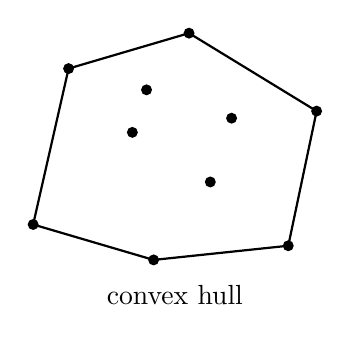
\begin{tikzpicture}[scale=.9]

\coordinate (A) at (-2,-1);
\coordinate (B) at (-1.5,1.2);
\coordinate (C) at (.2,1.7);
\coordinate (D) at (2,.6);
\coordinate (E) at (1.6,-1.3);
\coordinate (F) at (-.3,-1.5);

\draw[thick]
(A)--(B)--(C)--(D)--(E)--(F)--cycle;

\foreach \P in {A,B,C,D,E,F}
    \fill (\P) circle (2.2pt);

\fill (-.6,.3) circle (2.2pt);
\fill (.5,-.4) circle (2.2pt);
\fill (.8,.5) circle (2.2pt);
\fill (-.4,.9) circle (2.2pt);

\node at (0,-2) {convex hull};

\end{tikzpicture}
\end{centereddiagram}

%%%%%%%%%%%%%%%%%%%%%%%%%%%%%%%%%%%%%%%%%%%%%%%%%%%%%%%%%%%%
\subsection{Gift Wrapping}
\label{subsec:gift-wrapping}
%%%%%%%%%%%%%%%%%%%%%%%%%%%%%%%%%%%%%%%%%%%%%%%%%%%%%%%%%%%%

The \emph{gift-wrapping algorithm}, also called Jarvis march, constructs the
convex hull one edge at a time.

Beginning with an extreme point, the algorithm repeatedly selects the next
point so that all remaining points lie on the same side of the new hull
edge.

The process resembles wrapping a string around the point set.

If

\[
h
\]

is the number of hull vertices, the running time is

\[
\boxed{
O(nh).
}
\]

Thus the algorithm is output-sensitive.

%%%%%%%%%%%%%%%%%%%%%%%%%%%%%%%%%%%%%%%%%%%%%%%%%%%%%%%%%%%%
\subsection{Graham Scan}
\label{subsec:graham-scan}
%%%%%%%%%%%%%%%%%%%%%%%%%%%%%%%%%%%%%%%%%%%%%%%%%%%%%%%%%%%%

Graham scan is a classical convex-hull algorithm.

A simplified version proceeds as follows:

\begin{enumerate}
    \item choose a lowest point \(p_0\);
    \item sort the remaining points by polar angle around \(p_0\);
    \item process the sorted points in order;
    \item maintain a stack of candidate hull vertices;
    \item remove vertices whenever the stack makes an invalid turn.
\end{enumerate}

Orientation tests determine whether the current turn should remain on the
hull.

The sorting step dominates the running time:

\[
\boxed{
O(n\log n).
}
\]

%%%%%%%%%%%%%%%%%%%%%%%%%%%%%%%%%%%%%%%%%%%%%%%%%%%%%%%%%%%%
\subsection{Monotone Chain Convex Hull}
\label{subsec:monotone-chain-hull}
%%%%%%%%%%%%%%%%%%%%%%%%%%%%%%%%%%%%%%%%%%%%%%%%%%%%%%%%%%%%

The monotone chain algorithm first sorts points lexicographically, usually
by \(x\)-coordinate and then \(y\)-coordinate.

It then constructs:

\[
\boxed{
\text{lower hull}
}
\]

and

\[
\boxed{
\text{upper hull}.
}
\]

Orientation tests remove points that would create the wrong turn.

After sorting, each point is processed only a constant number of times.

Hence the total running time is

\[
\boxed{
O(n\log n).
}
\]

%%%%%%%%%%%%%%%%%%%%%%%%%%%%%%%%%%%%%%%%%%%%%%%%%%%%%%%%%%%%
\subsection{Worked Example: Hull Versus Interior Points}
\label{subsec:hull-interior-example}
%%%%%%%%%%%%%%%%%%%%%%%%%%%%%%%%%%%%%%%%%%%%%%%%%%%%%%%%%%%%

\begin{workedexamplebox}{Identify Convex-Hull Candidates}

Consider

\[
P=
\{
(0,0),
(4,0),
(4,3),
(0,3),
(2,1),
(2,2)
\}.
\]

The first four points form the corners of a rectangle.

The points

\[
(2,1)
\]

and

\[
(2,2)
\]

lie inside that rectangle.

Therefore they cannot be extreme points of the convex hull.

\begin{answerbox}
\[
\boxed{
\operatorname{conv}(P)
=
\operatorname{conv}
\{(0,0),(4,0),(4,3),(0,3)\}.
}
\]
\end{answerbox}
\end{workedexamplebox}

%%%%%%%%%%%%%%%%%%%%%%%%%%%%%%%%%%%%%%%%%%%%%%%%%%%%%%%%%%%%
\subsection{Point-in-Polygon Problems}
\label{subsec:point-in-polygon}
%%%%%%%%%%%%%%%%%%%%%%%%%%%%%%%%%%%%%%%%%%%%%%%%%%%%%%%%%%%%

Given a polygon \(P\) and a query point \(q\), the point-in-polygon problem
asks whether \(q\) lies

\[
\boxed{
\text{inside},
\quad
\text{outside},
\quad
\text{or on the boundary of }P.
}
\]

For convex polygons, the problem can exploit convexity.

For general simple polygons, ray-crossing and winding-number methods are
common.

%%%%%%%%%%%%%%%%%%%%%%%%%%%%%%%%%%%%%%%%%%%%%%%%%%%%%%%%%%%%
\subsection{Ray-Crossing Method}
\label{subsec:ray-crossing}
%%%%%%%%%%%%%%%%%%%%%%%%%%%%%%%%%%%%%%%%%%%%%%%%%%%%%%%%%%%%

Draw a ray beginning at the query point and extending indefinitely in a
fixed direction.

Under nondegenerate conditions:

\[
\boxed{
\text{odd number of boundary crossings}
\Longrightarrow
\text{inside},
}
\]

while

\[
\boxed{
\text{even number of boundary crossings}
\Longrightarrow
\text{outside}.
}
\]

Special care is required when the ray passes through polygon vertices or
overlaps polygon edges.

%%%%%%%%%%%%%%%%%%%%%%%%%%%%%%%%%%%%%%%%%%%%%%%%%%%%%%%%%%%%
\subsection{Winding Number}
\label{subsec:winding-number-computational}
%%%%%%%%%%%%%%%%%%%%%%%%%%%%%%%%%%%%%%%%%%%%%%%%%%%%%%%%%%%%

The winding number records how many times an oriented closed curve winds
around a point.

For a simple polygon and a point not on its boundary,

\[
\boxed{
\text{winding number}=0
}
\]

indicates that the point lies outside.

A nonzero winding number indicates that it lies inside.

This method generalizes more naturally to oriented curves.

%%%%%%%%%%%%%%%%%%%%%%%%%%%%%%%%%%%%%%%%%%%%%%%%%%%%%%%%%%%%
\subsection{Polygon Area: The Shoelace Formula}
\label{subsec:shoelace-formula}
%%%%%%%%%%%%%%%%%%%%%%%%%%%%%%%%%%%%%%%%%%%%%%%%%%%%%%%%%%%%

Let a simple polygon have vertices

\[
(x_1,y_1),\ldots,(x_n,y_n)
\]

listed cyclically.

Set

\[
(x_{n+1},y_{n+1})=(x_1,y_1).
\]

Then its area is

\[
\boxed{
A
=
\frac12
\left|
\sum_{i=1}^{n}
(x_i y_{i+1}-y_i x_{i+1})
\right|.
}
\]

This is commonly called the \emph{shoelace formula}.

%%%%%%%%%%%%%%%%%%%%%%%%%%%%%%%%%%%%%%%%%%%%%%%%%%%%%%%%%%%%
\subsection{Worked Example: Shoelace Formula}
\label{subsec:worked-shoelace}
%%%%%%%%%%%%%%%%%%%%%%%%%%%%%%%%%%%%%%%%%%%%%%%%%%%%%%%%%%%%

\begin{workedexamplebox}{Area of a Triangle}

Consider the triangle with vertices

\[
(0,0),
\qquad
(4,0),
\qquad
(1,3).
\]

Using the shoelace formula,

\[
A
=
\frac12
\left|
0\cdot0
+
4\cdot3
+
1\cdot0
-
0\cdot4
-
0\cdot1
-
3\cdot0
\right|.
\]

Therefore

\[
A
=
\frac12(12)
=
6.
\]

\begin{answerbox}
\[
\boxed{A=6}
\]
\end{answerbox}
\end{workedexamplebox}

%%%%%%%%%%%%%%%%%%%%%%%%%%%%%%%%%%%%%%%%%%%%%%%%%%%%%%%%%%%%
\subsection{Polygon Triangulation}
\label{subsec:computational-polygon-triangulation}
%%%%%%%%%%%%%%%%%%%%%%%%%%%%%%%%%%%%%%%%%%%%%%%%%%%%%%%%%%%%

Triangulation decomposes a polygon into triangles whose interiors do not
overlap.

A simple polygon with \(n\) vertices can be triangulated into

\[
\boxed{
n-2
}
\]

triangles using

\[
\boxed{
n-3
}
\]

noncrossing diagonals.

Triangulation is useful because many geometric computations are easier on
triangles than on arbitrary polygons.

%%%%%%%%%%%%%%%%%%%%%%%%%%%%%%%%%%%%%%%%%%%%%%%%%%%%%%%%%%%%
\subsection{Ear Clipping}
\label{subsec:ear-clipping}
%%%%%%%%%%%%%%%%%%%%%%%%%%%%%%%%%%%%%%%%%%%%%%%%%%%%%%%%%%%%

A common polygon-triangulation strategy is \emph{ear clipping}.

An \emph{ear} is formed by three consecutive polygon vertices such that:

\begin{itemize}
    \item the diagonal connecting the first and third vertices lies inside
    the polygon; and
    \item the corresponding triangle contains no other polygon vertex in its
    interior.
\end{itemize}

Removing ears one at a time eventually triangulates a simple polygon.

%%%%%%%%%%%%%%%%%%%%%%%%%%%%%%%%%%%%%%%%%%%%%%%%%%%%%%%%%%%%
\subsection{The Two-Ears Theorem}
\label{subsec:two-ears-theorem}
%%%%%%%%%%%%%%%%%%%%%%%%%%%%%%%%%%%%%%%%%%%%%%%%%%%%%%%%%%%%

\begin{theorem}[Two-Ears Theorem]
Every simple polygon with at least four vertices has at least two ears.
\end{theorem}

This theorem guarantees that the ear-clipping process always has a valid
next step.

%%%%%%%%%%%%%%%%%%%%%%%%%%%%%%%%%%%%%%%%%%%%%%%%%%%%%%%%%%%%
\subsection{Voronoi Diagrams}
\label{subsec:computational-voronoi}
%%%%%%%%%%%%%%%%%%%%%%%%%%%%%%%%%%%%%%%%%%%%%%%%%%%%%%%%%%%%

Given sites

\[
P=\{p_1,\ldots,p_n\},
\]

the Voronoi cell of \(p_i\) is

\[
\boxed{
V_i
=
\{
x:
\|x-p_i\|
\leq
\|x-p_j\|
\text{ for all }j
\}.
}
\]

The collection of these cells forms the Voronoi diagram.

Each cell contains the region for which its site is a nearest site.

%%%%%%%%%%%%%%%%%%%%%%%%%%%%%%%%%%%%%%%%%%%%%%%%%%%%%%%%%%%%
\subsection{Voronoi Boundaries}
\label{subsec:voronoi-boundaries-computational}
%%%%%%%%%%%%%%%%%%%%%%%%%%%%%%%%%%%%%%%%%%%%%%%%%%%%%%%%%%%%

For two sites \(p_i\) and \(p_j\), the points satisfying

\[
\|x-p_i\|
=
\|x-p_j\|
\]

lie on their perpendicular bisector.

Thus Voronoi cells are intersections of half-spaces and are convex in the
Euclidean setting.

%%%%%%%%%%%%%%%%%%%%%%%%%%%%%%%%%%%%%%%%%%%%%%%%%%%%%%%%%%%%
\subsection{Voronoi Vertices}
\label{subsec:voronoi-vertices}
%%%%%%%%%%%%%%%%%%%%%%%%%%%%%%%%%%%%%%%%%%%%%%%%%%%%%%%%%%%%

Under general-position assumptions, a planar Voronoi vertex is equidistant
from exactly three sites.

Those three sites lie on a common circle centered at the Voronoi vertex.

The interior of that circle contains no other site.

This observation leads directly to Delaunay triangulations.

%%%%%%%%%%%%%%%%%%%%%%%%%%%%%%%%%%%%%%%%%%%%%%%%%%%%%%%%%%%%
\subsection{Delaunay Triangulations}
\label{subsec:computational-delaunay}
%%%%%%%%%%%%%%%%%%%%%%%%%%%%%%%%%%%%%%%%%%%%%%%%%%%%%%%%%%%%

A planar Delaunay triangulation connects sites whose Voronoi cells share an
edge, assuming the standard nondegenerate setting.

The result is a geometric dual of the Voronoi diagram.

\[
\boxed{
\text{Voronoi edge}
\longleftrightarrow
\text{Delaunay edge}.
}
\]

%%%%%%%%%%%%%%%%%%%%%%%%%%%%%%%%%%%%%%%%%%%%%%%%%%%%%%%%%%%%
\subsection{Empty Circumcircle Criterion}
\label{subsec:empty-circumcircle-computational}
%%%%%%%%%%%%%%%%%%%%%%%%%%%%%%%%%%%%%%%%%%%%%%%%%%%%%%%%%%%%

For every triangle in a Delaunay triangulation,

\[
\boxed{
\text{the interior of its circumcircle contains no input site}.
}
\]

This is the empty circumcircle property.

If four sites lie on one circle, the Delaunay triangulation may not be
unique.

%%%%%%%%%%%%%%%%%%%%%%%%%%%%%%%%%%%%%%%%%%%%%%%%%%%%%%%%%%%%
\subsection{The In-Circle Predicate}
\label{subsec:incircle-predicate}
%%%%%%%%%%%%%%%%%%%%%%%%%%%%%%%%%%%%%%%%%%%%%%%%%%%%%%%%%%%%

Given four planar points \(a,b,c,d\), one may ask whether \(d\) lies inside
the circumcircle through \(a,b,c\).

For consistently oriented \(a,b,c\), this can be determined by the sign of

\[
\boxed{
\begin{vmatrix}
a_x & a_y & a_x^2+a_y^2 & 1\\
b_x & b_y & b_x^2+b_y^2 & 1\\
c_x & c_y & c_x^2+c_y^2 & 1\\
d_x & d_y & d_x^2+d_y^2 & 1
\end{vmatrix}.
}
\]

The sign convention depends on the orientation of \(a,b,c\).

This determinant is an important geometric predicate in Delaunay algorithms.

%%%%%%%%%%%%%%%%%%%%%%%%%%%%%%%%%%%%%%%%%%%%%%%%%%%%%%%%%%%%
\subsection{Delaunay Angle Property}
\label{subsec:delaunay-angle-property}
%%%%%%%%%%%%%%%%%%%%%%%%%%%%%%%%%%%%%%%%%%%%%%%%%%%%%%%%%%%%

Among triangulations of a planar point set in general position, the Delaunay
triangulation has a useful angle-quality property.

It maximizes the lexicographically sorted sequence of triangle angles and,
in particular, maximizes the minimum angle.

Thus Delaunay triangulations tend to avoid very thin triangles.

This makes them useful in mesh generation.

%%%%%%%%%%%%%%%%%%%%%%%%%%%%%%%%%%%%%%%%%%%%%%%%%%%%%%%%%%%%
\subsection{Nearest-Neighbor Queries}
\label{subsec:nearest-neighbor-query}
%%%%%%%%%%%%%%%%%%%%%%%%%%%%%%%%%%%%%%%%%%%%%%%%%%%%%%%%%%%%

Given a stored point set \(P\) and a query point \(q\), the nearest-neighbor
problem asks for

\[
\boxed{
p^*
=
\operatorname*{arg\,min}_{p\in P}
\|q-p\|.
}
\]

The symbol

\[
\operatorname*{arg\,min}
\]

is read ``argument of the minimum.''

It returns the input value where the minimum is achieved rather than the
minimum value itself.

%%%%%%%%%%%%%%%%%%%%%%%%%%%%%%%%%%%%%%%%%%%%%%%%%%%%%%%%%%%%
\subsection{Voronoi Diagrams and Nearest Neighbors}
\label{subsec:voronoi-nearest-neighbor}
%%%%%%%%%%%%%%%%%%%%%%%%%%%%%%%%%%%%%%%%%%%%%%%%%%%%%%%%%%%%

If a query point \(q\) lies inside the Voronoi cell \(V_i\), then

\[
\boxed{
p_i
}
\]

is a nearest site to \(q\).

Therefore Voronoi diagrams convert nearest-neighbor queries into
point-location problems.

%%%%%%%%%%%%%%%%%%%%%%%%%%%%%%%%%%%%%%%%%%%%%%%%%%%%%%%%%%%%
\subsection{Point Location}
\label{subsec:point-location}
%%%%%%%%%%%%%%%%%%%%%%%%%%%%%%%%%%%%%%%%%%%%%%%%%%%%%%%%%%%%

A planar subdivision divides the plane into vertices, edges, and faces.

The \emph{point-location problem} asks:

\[
\boxed{
\text{Which face contains a given query point?}
}
\]

Point location is a basic component of

\[
\boxed{
\text{GIS},
\quad
\text{computer graphics},
\quad
\text{mesh processing},
\quad
\text{Voronoi searching}.
}
\]

%%%%%%%%%%%%%%%%%%%%%%%%%%%%%%%%%%%%%%%%%%%%%%%%%%%%%%%%%%%%
\subsection{Range Searching}
\label{subsec:range-searching}
%%%%%%%%%%%%%%%%%%%%%%%%%%%%%%%%%%%%%%%%%%%%%%%%%%%%%%%%%%%%

Suppose a point set

\[
P\subseteq\R^d
\]

is stored.

A range query asks for all points lying inside a specified region \(R\):

\[
\boxed{
P\cap R.
}
\]

Typical ranges include:

\[
\boxed{
\text{rectangles},
\quad
\text{boxes},
\quad
\text{circles},
\quad
\text{half-spaces}.
}
\]

%%%%%%%%%%%%%%%%%%%%%%%%%%%%%%%%%%%%%%%%%%%%%%%%%%%%%%%%%%%%
\subsection{Orthogonal Range Searching}
\label{subsec:orthogonal-range-searching}
%%%%%%%%%%%%%%%%%%%%%%%%%%%%%%%%%%%%%%%%%%%%%%%%%%%%%%%%%%%%

In orthogonal range searching, query regions are axis-aligned rectangles or
higher-dimensional boxes.

For example,

\[
R=
[a_1,b_1]\times\cdots\times[a_d,b_d].
\]

The goal is to report or count points satisfying

\[
\boxed{
a_i\leq x_i\leq b_i
}
\]

for every coordinate \(i\).

%%%%%%%%%%%%%%%%%%%%%%%%%%%%%%%%%%%%%%%%%%%%%%%%%%%%%%%%%%%%
\subsection{\texorpdfstring{\(k\)-d Trees}{k-d Trees}}
\label{subsec:kd-trees}
%%%%%%%%%%%%%%%%%%%%%%%%%%%%%%%%%%%%%%%%%%%%%%%%%%%%%%%%%%%%

A \(k\)-d tree is a hierarchical spatial data structure.

The letter \(k\) refers to the number of coordinate dimensions.

At each stage, the data are divided using a coordinate-aligned hyperplane.

In two dimensions, the algorithm may alternate between

\[
\boxed{x\text{-splits}}
\]

and

\[
\boxed{y\text{-splits}}.
\]

%%%%%%%%%%%%%%%%%%%%%%%%%%%%%%%%%%%%%%%%%%%%%%%%%%%%%%%%%%%%
\subsection{Schematic \texorpdfstring{\(k\)-d}{k-d} Partition}
\label{subsec:kd-partition}
%%%%%%%%%%%%%%%%%%%%%%%%%%%%%%%%%%%%%%%%%%%%%%%%%%%%%%%%%%%%

\begin{centereddiagram}
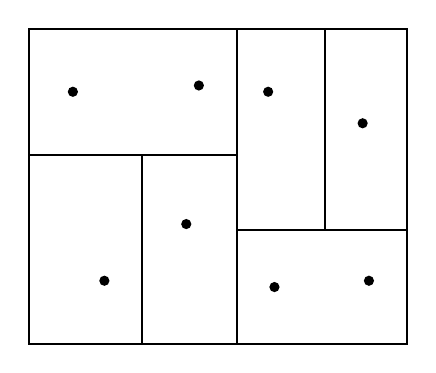
\begin{tikzpicture}[scale=.8]

\draw[thick] (-3,-2.5) rectangle (3,2.5);

\draw[thick] (.3,-2.5)--(.3,2.5);
\draw[thick] (-3,.5)--(.3,.5);
\draw[thick] (.3,-.7)--(3,-.7);
\draw[thick] (-1.2,-2.5)--(-1.2,.5);
\draw[thick] (1.7,-.7)--(1.7,2.5);

\foreach \p in {
(-2.3,1.5),
(-1.8,-1.5),
(-.5,-.6),
(-.3,1.6),
(.8,1.5),
(2.3,1),
(.9,-1.6),
(2.4,-1.5)
}{
\fill \p circle (2.3pt);
}

\end{tikzpicture}
\end{centereddiagram}

The diagram illustrates recursive axis-aligned subdivision rather than one
unique \(k\)-d tree.

%%%%%%%%%%%%%%%%%%%%%%%%%%%%%%%%%%%%%%%%%%%%%%%%%%%%%%%%%%%%
\subsection{Quadtrees}
\label{subsec:quadtrees}
%%%%%%%%%%%%%%%%%%%%%%%%%%%%%%%%%%%%%%%%%%%%%%%%%%%%%%%%%%%%

A quadtree recursively divides a two-dimensional region into four
subregions.

Each subdivision produces four children.

The three-dimensional analogue is an \emph{octree}, which divides a region
into eight subregions.

These structures are useful when geometric data are distributed
nonuniformly through space.

%%%%%%%%%%%%%%%%%%%%%%%%%%%%%%%%%%%%%%%%%%%%%%%%%%%%%%%%%%%%
\subsection{Bounding-Volume Hierarchies}
\label{subsec:bounding-volume-hierarchies}
%%%%%%%%%%%%%%%%%%%%%%%%%%%%%%%%%%%%%%%%%%%%%%%%%%%%%%%%%%%%

A bounding-volume hierarchy groups geometric objects inside simple enclosing
regions.

Possible bounding volumes include

\[
\boxed{
\text{axis-aligned boxes},
\quad
\text{oriented boxes},
\quad
\text{spheres}.
}
\]

If two bounding volumes do not intersect, then none of the objects contained
within them can intersect.

This permits large groups of objects to be rejected at once.

%%%%%%%%%%%%%%%%%%%%%%%%%%%%%%%%%%%%%%%%%%%%%%%%%%%%%%%%%%%%
\subsection{Collision Detection}
\label{subsec:collision-detection}
%%%%%%%%%%%%%%%%%%%%%%%%%%%%%%%%%%%%%%%%%%%%%%%%%%%%%%%%%%%%

Collision detection asks whether moving or stationary geometric objects
intersect.

A typical strategy has two stages:

\[
\boxed{
\text{broad phase}
\longrightarrow
\text{narrow phase}.
}
\]

The broad phase quickly eliminates pairs that clearly cannot collide.

The narrow phase performs more accurate geometric intersection tests on the
remaining candidates.

%%%%%%%%%%%%%%%%%%%%%%%%%%%%%%%%%%%%%%%%%%%%%%%%%%%%%%%%%%%%
\subsection{Sweep-Line Algorithms}
\label{subsec:sweep-line-algorithms}
%%%%%%%%%%%%%%%%%%%%%%%%%%%%%%%%%%%%%%%%%%%%%%%%%%%%%%%%%%%%

A \emph{sweep-line algorithm} imagines moving a line across the plane.

The algorithm processes geometric events in the order in which the sweep
line encounters them.

Usually it maintains:

\[
\boxed{
\text{an event queue}
}
\]

and

\[
\boxed{
\text{a dynamic status structure}.
}
\]

This converts a two-dimensional geometric problem into a sequence of
one-dimensional updates.

%%%%%%%%%%%%%%%%%%%%%%%%%%%%%%%%%%%%%%%%%%%%%%%%%%%%%%%%%%%%
\subsection{Segment Intersection by Sweeping}
\label{subsec:sweep-segment-intersection}
%%%%%%%%%%%%%%%%%%%%%%%%%%%%%%%%%%%%%%%%%%%%%%%%%%%%%%%%%%%%

Suppose many line segments are given.

Checking every pair requires

\[
O(n^2)
\]

intersection tests.

A sweep-line algorithm instead processes segment endpoints and intersection
events while maintaining the vertical ordering of segments crossing the
sweep line.

This can dramatically reduce unnecessary comparisons.

%%%%%%%%%%%%%%%%%%%%%%%%%%%%%%%%%%%%%%%%%%%%%%%%%%%%%%%%%%%%
\subsection{Bentley--Ottmann Algorithm}
\label{subsec:bentley-ottmann}
%%%%%%%%%%%%%%%%%%%%%%%%%%%%%%%%%%%%%%%%%%%%%%%%%%%%%%%%%%%%

The Bentley--Ottmann algorithm reports intersections among planar line
segments using a sweep line.

For \(n\) segments and \(k\) reported intersections, a standard bound is

\[
\boxed{
O((n+k)\log n).
}
\]

This is an example of an \emph{output-sensitive algorithm}, because the
running time depends partly on the number of intersections actually found.

%%%%%%%%%%%%%%%%%%%%%%%%%%%%%%%%%%%%%%%%%%%%%%%%%%%%%%%%%%%%
\subsection{Output-Sensitive Algorithms}
\label{subsec:output-sensitive-geometry}
%%%%%%%%%%%%%%%%%%%%%%%%%%%%%%%%%%%%%%%%%%%%%%%%%%%%%%%%%%%%

An algorithm is output-sensitive when its complexity depends on both the
input size and output size.

For example, Jarvis march computes a planar convex hull in

\[
\boxed{
O(nh),
}
\]

where

\[
h
\]

is the number of hull vertices.

This can be advantageous when

\[
h\ll n.
\]

%%%%%%%%%%%%%%%%%%%%%%%%%%%%%%%%%%%%%%%%%%%%%%%%%%%%%%%%%%%%
\subsection{Arrangements}
\label{subsec:geometric-arrangements}
%%%%%%%%%%%%%%%%%%%%%%%%%%%%%%%%%%%%%%%%%%%%%%%%%%%%%%%%%%%%

An \emph{arrangement} is the subdivision of space produced by a collection
of geometric objects.

For example, a collection of lines in the plane divides the plane into

\[
\boxed{
\text{vertices},
\quad
\text{edges},
\quad
\text{faces}.
}
\]

Arrangement theory studies the combinatorial complexity of these
subdivisions and algorithms for constructing them.

%%%%%%%%%%%%%%%%%%%%%%%%%%%%%%%%%%%%%%%%%%%%%%%%%%%%%%%%%%%%
\subsection{Arrangement of Lines}
\label{subsec:arrangement-lines}
%%%%%%%%%%%%%%%%%%%%%%%%%%%%%%%%%%%%%%%%%%%%%%%%%%%%%%%%%%%%

Suppose \(n\) lines are in general position in the plane, meaning:

\begin{itemize}
    \item no two are parallel;
    \item no three pass through one point.
\end{itemize}

Then the number of intersection vertices is

\[
\boxed{
\binom{n}{2}.
}
\]

The maximum number of regions formed is

\[
\boxed{
1+\frac{n(n+1)}{2}.
}
\]

This is a simple example of combinatorial complexity arising from geometry.

%%%%%%%%%%%%%%%%%%%%%%%%%%%%%%%%%%%%%%%%%%%%%%%%%%%%%%%%%%%%
\subsection{Visibility Problems}
\label{subsec:visibility-problems}
%%%%%%%%%%%%%%%%%%%%%%%%%%%%%%%%%%%%%%%%%%%%%%%%%%%%%%%%%%%%

Two points in a region are mutually visible if the segment joining them lies
entirely within the allowed region.

Visibility problems arise in

\[
\boxed{
\text{robotics},
\quad
\text{graphics},
\quad
\text{surveillance},
\quad
\text{motion planning}.
}
\]

%%%%%%%%%%%%%%%%%%%%%%%%%%%%%%%%%%%%%%%%%%%%%%%%%%%%%%%%%%%%
\subsection{Visibility Graphs}
\label{subsec:visibility-graphs}
%%%%%%%%%%%%%%%%%%%%%%%%%%%%%%%%%%%%%%%%%%%%%%%%%%%%%%%%%%%%

For polygonal obstacles, one may construct a graph whose vertices include
obstacle vertices together with start and goal points.

Two vertices are connected when the segment joining them does not pass
through an obstacle interior.

The resulting \emph{visibility graph} can convert a geometric shortest-path
problem into a graph shortest-path problem.

%%%%%%%%%%%%%%%%%%%%%%%%%%%%%%%%%%%%%%%%%%%%%%%%%%%%%%%%%%%%
\subsection{Shortest Paths Among Obstacles}
\label{subsec:shortest-path-obstacles}
%%%%%%%%%%%%%%%%%%%%%%%%%%%%%%%%%%%%%%%%%%%%%%%%%%%%%%%%%%%%

Suppose a point must travel from

\[
s
\]

to

\[
t
\]

while avoiding polygonal obstacles.

The objective is to minimize path length.

For polygonal obstacles in the plane, shortest paths bend only where
necessary, typically at obstacle vertices.

This creates a close connection between geometry and graph algorithms.

%%%%%%%%%%%%%%%%%%%%%%%%%%%%%%%%%%%%%%%%%%%%%%%%%%%%%%%%%%%%
\subsection{Motion Planning}
\label{subsec:motion-planning}
%%%%%%%%%%%%%%%%%%%%%%%%%%%%%%%%%%%%%%%%%%%%%%%%%%%%%%%%%%%%

Robotics introduces an additional complication: the moving object may have
nonzero size and may rotate.

Rather than moving the entire robot directly, one can describe its
configuration using a point in a higher-dimensional
\emph{configuration space}.

Then the motion-planning problem becomes:

\[
\boxed{
\text{find a path through collision-free configuration space}.
}
\]

%%%%%%%%%%%%%%%%%%%%%%%%%%%%%%%%%%%%%%%%%%%%%%%%%%%%%%%%%%%%
\subsection{Configuration Spaces}
\label{subsec:configuration-spaces}
%%%%%%%%%%%%%%%%%%%%%%%%%%%%%%%%%%%%%%%%%%%%%%%%%%%%%%%%%%%%

A configuration records all parameters needed to describe the position of a
mechanical system.

For a translating point in the plane,

\[
\boxed{
\text{configuration space}=\R^2.
}
\]

For a rigid planar body that can translate and rotate, a configuration may
be described by

\[
\boxed{
(x,y,\theta),
}
\]

where \(\theta\), read ``theta,'' represents orientation.

Configuration-space ideas connect computational geometry with topology and
robotics.

%%%%%%%%%%%%%%%%%%%%%%%%%%%%%%%%%%%%%%%%%%%%%%%%%%%%%%%%%%%%
\subsection{Minkowski Sums in Motion Planning}
\label{subsec:minkowski-motion-planning}
%%%%%%%%%%%%%%%%%%%%%%%%%%%%%%%%%%%%%%%%%%%%%%%%%%%%%%%%%%%%

Minkowski sums, introduced in Convex Geometry, are useful for handling
objects with nonzero size.

For sets \(A\) and \(B\),

\[
A+B
=
\{a+b:a\in A,\ b\in B\}.
\]

By expanding obstacles according to the robot's shape, a moving-body problem
can often be transformed into an equivalent point-motion problem.

This is sometimes described as constructing configuration-space obstacles.

%%%%%%%%%%%%%%%%%%%%%%%%%%%%%%%%%%%%%%%%%%%%%%%%%%%%%%%%%%%%
\subsection{Meshes}
\label{subsec:computational-meshes}
%%%%%%%%%%%%%%%%%%%%%%%%%%%%%%%%%%%%%%%%%%%%%%%%%%%%%%%%%%%%

A mesh approximates a geometric domain using simple cells.

In two dimensions, triangular meshes are common.

In three dimensions, tetrahedral meshes are frequently used.

Meshes are central to

\[
\boxed{
\text{finite element methods},
\quad
\text{computer graphics},
\quad
\text{scientific simulation}.
}
\]

%%%%%%%%%%%%%%%%%%%%%%%%%%%%%%%%%%%%%%%%%%%%%%%%%%%%%%%%%%%%
\subsection{Mesh Quality}
\label{subsec:mesh-quality}
%%%%%%%%%%%%%%%%%%%%%%%%%%%%%%%%%%%%%%%%%%%%%%%%%%%%%%%%%%%%

Not all triangulations are equally useful numerically.

Very thin triangles can lead to poor numerical behavior.

Mesh-generation algorithms therefore attempt to control quantities such as

\[
\boxed{
\text{minimum angle},
\quad
\text{aspect ratio},
\quad
\text{element size}.
}
\]

The favorable angle properties of Delaunay triangulations make them
especially important in mesh generation.

%%%%%%%%%%%%%%%%%%%%%%%%%%%%%%%%%%%%%%%%%%%%%%%%%%%%%%%%%%%%
\subsection{Geometric Optimization}
\label{subsec:geometric-optimization}
%%%%%%%%%%%%%%%%%%%%%%%%%%%%%%%%%%%%%%%%%%%%%%%%%%%%%%%%%%%%

Many computational geometry problems are optimization problems.

Examples include:

\[
\boxed{
\min_{p_i\neq p_j}
\|p_i-p_j\|
}
\]

for the closest pair,

\[
\boxed{
\min_{p\in P}
\|q-p\|
}
\]

for nearest-neighbor search, and

\[
\boxed{
\min_{\gamma}
L(\gamma)
}
\]

for shortest-path problems.

Thus computational geometry interacts naturally with mathematical
optimization.

%%%%%%%%%%%%%%%%%%%%%%%%%%%%%%%%%%%%%%%%%%%%%%%%%%%%%%%%%%%%
\subsection{The Smallest Enclosing Circle}
\label{subsec:smallest-enclosing-circle}
%%%%%%%%%%%%%%%%%%%%%%%%%%%%%%%%%%%%%%%%%%%%%%%%%%%%%%%%%%%%

Given a finite planar point set \(P\), the smallest enclosing circle problem
asks for a circle of minimum radius containing every point.

The solution is determined by a small subset of boundary points.

In the nondegenerate planar case, the optimal circle is typically determined
by either

\[
\boxed{
\text{two diametrically opposite boundary points}
}
\]

or

\[
\boxed{
\text{three boundary points defining the circle}.
}
\]

%%%%%%%%%%%%%%%%%%%%%%%%%%%%%%%%%%%%%%%%%%%%%%%%%%%%%%%%%%%%
\subsection{Geometric Duality}
\label{subsec:computational-geometric-duality}
%%%%%%%%%%%%%%%%%%%%%%%%%%%%%%%%%%%%%%%%%%%%%%%%%%%%%%%%%%%%

Geometric duality can transform one type of geometric object into another.

For example, under a suitable point-line duality, a point

\[
p=(a,b)
\]

may correspond to a line such as

\[
\boxed{
y=ax-b.
}
\]

Conversely, a nonvertical line

\[
y=mx-c
\]

corresponds to the point

\[
\boxed{
(m,c).
}
\]

Different duality conventions are possible.

%%%%%%%%%%%%%%%%%%%%%%%%%%%%%%%%%%%%%%%%%%%%%%%%%%%%%%%%%%%%
\subsection{Why Duality Is Useful}
\label{subsec:why-computational-duality}
%%%%%%%%%%%%%%%%%%%%%%%%%%%%%%%%%%%%%%%%%%%%%%%%%%%%%%%%%%%%

A difficult problem involving points may become easier after conversion into
a problem involving lines.

For example,

\[
\boxed{
\text{point-line incidences}
}
\]

may be transformed into

\[
\boxed{
\text{dual line-point incidences}.
}
\]

Duality is therefore both a theoretical and algorithmic technique.

%%%%%%%%%%%%%%%%%%%%%%%%%%%%%%%%%%%%%%%%%%%%%%%%%%%%%%%%%%%%
\subsection{Randomized Geometric Algorithms}
\label{subsec:randomized-geometric-algorithms}
%%%%%%%%%%%%%%%%%%%%%%%%%%%%%%%%%%%%%%%%%%%%%%%%%%%%%%%%%%%%

Randomization can simplify geometric algorithms.

A randomized incremental algorithm processes objects in random order and
updates the geometric structure as each object is inserted.

This approach is used in algorithms for structures such as

\[
\boxed{
\text{convex hulls},
\quad
\text{Delaunay triangulations},
\quad
\text{arrangements}.
}
\]

Expected running-time analysis is then performed using probability.

%%%%%%%%%%%%%%%%%%%%%%%%%%%%%%%%%%%%%%%%%%%%%%%%%%%%%%%%%%%%
\subsection{Degeneracy}
\label{subsec:computational-degeneracy}
%%%%%%%%%%%%%%%%%%%%%%%%%%%%%%%%%%%%%%%%%%%%%%%%%%%%%%%%%%%%

A geometric input is \emph{degenerate} when special coincidences occur.

Examples include:

\[
\boxed{
\text{three collinear points},
}
\]

\[
\boxed{
\text{four cocircular points},
}
\]

\[
\boxed{
\text{overlapping segments},
}
\]

\[
\boxed{
\text{multiple events at the same coordinate}.
}
\]

These cases often require additional algorithmic logic.

%%%%%%%%%%%%%%%%%%%%%%%%%%%%%%%%%%%%%%%%%%%%%%%%%%%%%%%%%%%%
\subsection{General Position Assumptions}
\label{subsec:computational-general-position}
%%%%%%%%%%%%%%%%%%%%%%%%%%%%%%%%%%%%%%%%%%%%%%%%%%%%%%%%%%%%

To simplify theoretical analysis, algorithms are often first described under
general-position assumptions.

Examples include:

\[
\boxed{
\text{no three points collinear}
}
\]

or

\[
\boxed{
\text{no four points cocircular}.
}
\]

These assumptions remove degeneracies.

However, practical software must eventually decide how such cases are
handled.

%%%%%%%%%%%%%%%%%%%%%%%%%%%%%%%%%%%%%%%%%%%%%%%%%%%%%%%%%%%%
\subsection{Exact Versus Floating-Point Arithmetic}
\label{subsec:exact-floating-geometry}
%%%%%%%%%%%%%%%%%%%%%%%%%%%%%%%%%%%%%%%%%%%%%%%%%%%%%%%%%%%%

A mathematical orientation determinant may equal exactly zero.

A computer using floating-point arithmetic may instead obtain a very small
positive or negative value because of rounding error.

Thus

\[
\boxed{
\text{mathematically exact predicate}
}
\]

and

\[
\boxed{
\text{numerically computed predicate}
}
\]

are not automatically the same.

%%%%%%%%%%%%%%%%%%%%%%%%%%%%%%%%%%%%%%%%%%%%%%%%%%%%%%%%%%%%
\subsection{Robust Geometric Computation}
\label{subsec:robust-geometric-computation}
%%%%%%%%%%%%%%%%%%%%%%%%%%%%%%%%%%%%%%%%%%%%%%%%%%%%%%%%%%%%

A geometric algorithm is \emph{robust} when it behaves correctly even in
the presence of numerical error and degenerate inputs.

Common strategies include:

\begin{itemize}
    \item exact arithmetic;
    \item adaptive-precision arithmetic;
    \item carefully designed robust predicates;
    \item symbolic perturbation;
    \item explicit degeneracy handling.
\end{itemize}

\begin{importantbox}
In computational geometry, a theoretically correct algorithm can still fail
in software if its geometric predicates are evaluated unreliably.
\end{importantbox}

%%%%%%%%%%%%%%%%%%%%%%%%%%%%%%%%%%%%%%%%%%%%%%%%%%%%%%%%%%%%
\subsection{Symbolic Perturbation}
\label{subsec:symbolic-perturbation}
%%%%%%%%%%%%%%%%%%%%%%%%%%%%%%%%%%%%%%%%%%%%%%%%%%%%%%%%%%%%

Symbolic perturbation conceptually moves input objects by infinitesimally
small amounts so that degeneracies disappear.

The perturbation is not necessarily performed numerically.

Instead, the algorithm uses a consistent rule that behaves as if the input
had been slightly perturbed.

This allows general-position reasoning while preserving deterministic
behavior.

%%%%%%%%%%%%%%%%%%%%%%%%%%%%%%%%%%%%%%%%%%%%%%%%%%%%%%%%%%%%
\subsection{Higher-Dimensional Computational Geometry}
\label{subsec:higher-dimensional-computational-geometry}
%%%%%%%%%%%%%%%%%%%%%%%%%%%%%%%%%%%%%%%%%%%%%%%%%%%%%%%%%%%%

Many planar problems extend to

\[
\R^d.
\]

Examples include:

\[
\boxed{
\text{convex hulls},
\quad
\text{Voronoi diagrams},
\quad
\text{nearest neighbors},
\quad
\text{range searching}.
}
\]

However, computational complexity often increases rapidly with dimension.

%%%%%%%%%%%%%%%%%%%%%%%%%%%%%%%%%%%%%%%%%%%%%%%%%%%%%%%%%%%%
\subsection{The Curse of Dimensionality}
\label{subsec:geometry-curse-dimensionality}
%%%%%%%%%%%%%%%%%%%%%%%%%%%%%%%%%%%%%%%%%%%%%%%%%%%%%%%%%%%%

Algorithms that perform well in two or three dimensions may become
inefficient in high dimensions.

This phenomenon is commonly associated with the
\emph{curse of dimensionality}.

For example, spatial partitions may become less selective as dimension
increases, while combinatorial complexity can grow rapidly.

This is especially important in high-dimensional data analysis.

%%%%%%%%%%%%%%%%%%%%%%%%%%%%%%%%%%%%%%%%%%%%%%%%%%%%%%%%%%%%
\subsection{Applications to Geographic Information Systems}
\label{subsec:computational-geometry-gis}
%%%%%%%%%%%%%%%%%%%%%%%%%%%%%%%%%%%%%%%%%%%%%%%%%%%%%%%%%%%%

Geographic information systems, or GIS, manipulate spatial data such as

\[
\boxed{
\text{roads},
\quad
\text{parcels},
\quad
\text{boundaries},
\quad
\text{elevation},
\quad
\text{service regions}.
}
\]

Computational geometry provides algorithms for

\[
\boxed{
\text{intersection},
\quad
\text{point location},
\quad
\text{nearest neighbors},
\quad
\text{spatial indexing}.
}
\]

%%%%%%%%%%%%%%%%%%%%%%%%%%%%%%%%%%%%%%%%%%%%%%%%%%%%%%%%%%%%
\subsection{Applications to Computer Graphics}
\label{subsec:computational-geometry-graphics}
%%%%%%%%%%%%%%%%%%%%%%%%%%%%%%%%%%%%%%%%%%%%%%%%%%%%%%%%%%%%

Computer graphics relies heavily on geometric computation.

Examples include:

\[
\boxed{
\text{mesh construction},
}
\]

\[
\boxed{
\text{ray intersection},
}
\]

\[
\boxed{
\text{visibility},
}
\]

\[
\boxed{
\text{collision detection},
}
\]

\[
\boxed{
\text{surface approximation}.
}
\]

Bounding-volume hierarchies and spatial subdivisions are particularly
important for accelerating large geometric queries.

%%%%%%%%%%%%%%%%%%%%%%%%%%%%%%%%%%%%%%%%%%%%%%%%%%%%%%%%%%%%
\subsection{Applications to Robotics}
\label{subsec:computational-geometry-robotics}
%%%%%%%%%%%%%%%%%%%%%%%%%%%%%%%%%%%%%%%%%%%%%%%%%%%%%%%%%%%%

Robotics uses computational geometry for

\[
\boxed{
\text{motion planning},
\quad
\text{collision avoidance},
\quad
\text{localization},
\quad
\text{mapping}.
}
\]

Configuration spaces transform robot motion into geometric path problems.

Voronoi structures can also help construct paths that remain far from
obstacles.

%%%%%%%%%%%%%%%%%%%%%%%%%%%%%%%%%%%%%%%%%%%%%%%%%%%%%%%%%%%%
\subsection{Applications to Data Analysis}
\label{subsec:computational-geometry-data}
%%%%%%%%%%%%%%%%%%%%%%%%%%%%%%%%%%%%%%%%%%%%%%%%%%%%%%%%%%%%

Data points in

\[
\R^d
\]

can be studied geometrically.

Computational tools include:

\[
\boxed{
\text{nearest neighbors},
\quad
\text{convex hulls},
\quad
\text{spatial partitions},
\quad
\text{proximity graphs}.
}
\]

These ideas appear in classification, clustering, anomaly detection, and
geometric data analysis.

%%%%%%%%%%%%%%%%%%%%%%%%%%%%%%%%%%%%%%%%%%%%%%%%%%%%%%%%%%%%
\subsection{Applications to Scientific Computing}
\label{subsec:computational-geometry-scientific-computing}
%%%%%%%%%%%%%%%%%%%%%%%%%%%%%%%%%%%%%%%%%%%%%%%%%%%%%%%%%%%%

Scientific simulations often require geometric preprocessing.

A physical domain may first be converted into a mesh.

Differential equations are then approximated on that mesh using methods such
as finite elements.

Thus a pipeline may have the form

\[
\boxed{
\text{geometry}
\longrightarrow
\text{mesh}
\longrightarrow
\text{numerical model}
\longrightarrow
\text{simulation}.
}
\]

%%%%%%%%%%%%%%%%%%%%%%%%%%%%%%%%%%%%%%%%%%%%%%%%%%%%%%%%%%%%
\subsection{Common Errors}
\label{subsec:computational-geometry-common-errors}
%%%%%%%%%%%%%%%%%%%%%%%%%%%%%%%%%%%%%%%%%%%%%%%%%%%%%%%%%%%%

\subsubsection{Confusing Mathematical Geometry with Computational Geometry}

Computational geometry is not simply geometry performed with a calculator.

The subject studies algorithms, complexity, data structures, numerical
reliability, and geometric representations.

%%%%%%%%%%%%%%%%%%%%%%%%%%%%%%%%%%%%%%%%%%%%%%%%%%%%%%%%%%%%
\subsubsection{Using Slope When a Determinant Is Better}

Slope calculations can fail for vertical lines and may require division.

Orientation determinants avoid division and treat all directions uniformly.

Thus

\[
\boxed{
\operatorname{orient}(p,q,r)
}
\]

is usually preferable to comparing slopes.

%%%%%%%%%%%%%%%%%%%%%%%%%%%%%%%%%%%%%%%%%%%%%%%%%%%%%%%%%%%%
\subsubsection{Taking Square Roots Unnecessarily}

To determine whether

\[
d(p,q)<d(p,r),
\]

it is enough to compare

\[
\boxed{
d^2(p,q)<d^2(p,r).
}
\]

The square root need not be computed.

%%%%%%%%%%%%%%%%%%%%%%%%%%%%%%%%%%%%%%%%%%%%%%%%%%%%%%%%%%%%
\subsubsection{Ignoring Collinear Cases in Segment Intersection}

The strict orientation test detects proper crossings.

Endpoint contact and collinear overlap require additional tests.

%%%%%%%%%%%%%%%%%%%%%%%%%%%%%%%%%%%%%%%%%%%%%%%%%%%%%%%%%%%%
\subsubsection{Assuming Every Point Belongs on the Convex Hull}

Interior points do not appear as convex-hull vertices.

Only extreme boundary points are required.

%%%%%%%%%%%%%%%%%%%%%%%%%%%%%%%%%%%%%%%%%%%%%%%%%%%%%%%%%%%%
\subsubsection{Assuming Every Convex-Hull Algorithm Is Quadratic}

Efficient planar convex-hull algorithms achieve

\[
\boxed{
O(n\log n)
}
\]

running time.

Output-sensitive algorithms may perform differently depending on the number
of hull vertices.

%%%%%%%%%%%%%%%%%%%%%%%%%%%%%%%%%%%%%%%%%%%%%%%%%%%%%%%%%%%%
\subsubsection{Assuming Delaunay Triangulations Are Always Unique}

Four cocircular sites can produce multiple valid Delaunay triangulations.

Uniqueness follows under suitable general-position assumptions.

%%%%%%%%%%%%%%%%%%%%%%%%%%%%%%%%%%%%%%%%%%%%%%%%%%%%%%%%%%%%
\subsubsection{Confusing Voronoi and Delaunay Structures}

Voronoi diagrams partition space into nearest-site regions.

Delaunay triangulations connect sites according to adjacency of their
Voronoi cells.

They are dual structures, not the same structure.

%%%%%%%%%%%%%%%%%%%%%%%%%%%%%%%%%%%%%%%%%%%%%%%%%%%%%%%%%%%%
\subsubsection{Ignoring Polygon Orientation}

The sign of a signed-area or orientation calculation depends on vertex
ordering.

Clockwise and counterclockwise orderings produce opposite signs.

%%%%%%%%%%%%%%%%%%%%%%%%%%%%%%%%%%%%%%%%%%%%%%%%%%%%%%%%%%%%
\subsubsection{Assuming Floating-Point Zero Means Exact Zero}

A computed value such as

\[
10^{-14}
\]

may represent numerical error rather than genuine geometric separation.

Robust predicates require more care than simply checking approximate values.

%%%%%%%%%%%%%%%%%%%%%%%%%%%%%%%%%%%%%%%%%%%%%%%%%%%%%%%%%%%%
\subsubsection{Using an Arbitrary Tolerance Everywhere}

Replacing every comparison with a fixed tolerance does not automatically
make a geometric algorithm robust.

The appropriate numerical scale can vary greatly between problems.

%%%%%%%%%%%%%%%%%%%%%%%%%%%%%%%%%%%%%%%%%%%%%%%%%%%%%%%%%%%%
\subsubsection{Ignoring Degenerate Input}

Real data can contain

\[
\boxed{
\text{duplicates},
\quad
\text{collinearities},
\quad
\text{cocircularities},
\quad
\text{overlaps}.
}
\]

A practical algorithm should specify how these cases are treated.

%%%%%%%%%%%%%%%%%%%%%%%%%%%%%%%%%%%%%%%%%%%%%%%%%%%%%%%%%%%%
\subsubsection{Confusing Worst-Case and Expected Complexity}

A randomized algorithm may have good expected running time without having
the same worst-case bound.

The type of complexity statement must be identified.

%%%%%%%%%%%%%%%%%%%%%%%%%%%%%%%%%%%%%%%%%%%%%%%%%%%%%%%%%%%%
\subsubsection{Assuming Low-Dimensional Methods Scale Directly}

An algorithm that is excellent in \(\R^2\) may become impractical in high
dimensions.

Dimensional dependence is an essential part of geometric algorithm design.

%%%%%%%%%%%%%%%%%%%%%%%%%%%%%%%%%%%%%%%%%%%%%%%%%%%%%%%%%%%%
\subsection{Applications and Connections}
\label{subsec:computational-geometry-applications}
%%%%%%%%%%%%%%%%%%%%%%%%%%%%%%%%%%%%%%%%%%%%%%%%%%%%%%%%%%%%

\begin{applicationbox}
\textbf{Convex Geometry.}
Convex-hull algorithms turn the theoretical convex hull into an explicit
computational object.

\medskip

\textbf{Discrete Geometry.}
Point configurations, Voronoi diagrams, Delaunay triangulations, packings,
polytopes, and geometric graphs provide many of the basic inputs and
structures studied algorithmically.

\medskip

\textbf{Linear Algebra.}
Determinants, vector products, linear systems, and transformations provide
many of the fundamental computational predicates.

\medskip

\textbf{Algorithms and Data Structures.}
Sorting, divide and conquer, balanced trees, spatial partitions, priority
queues, and randomized algorithms are central computational tools.

\medskip

\textbf{Optimization.}
Closest-pair, nearest-neighbor, enclosing-shape, and shortest-path problems
are geometric optimization problems.

\medskip

\textbf{Computer Graphics.}
Ray intersection, meshes, collision detection, visibility, and spatial
acceleration structures are geometric algorithm problems.

\medskip

\textbf{Robotics.}
Motion planning, configuration spaces, obstacle avoidance, and localization
depend on geometric computation.

\medskip

\textbf{GIS.}
Spatial indexing, overlay operations, point location, nearest facilities,
and region queries use computational geometry extensively.

\medskip

\textbf{Scientific Computing.}
Mesh generation provides geometric discretizations for numerical methods
such as finite element analysis.

\medskip

\textbf{Data Science.}
Nearest-neighbor search, spatial trees, geometric classification, and
high-dimensional proximity problems connect computational geometry with
modern data analysis.
\end{applicationbox}

%%%%%%%%%%%%%%%%%%%%%%%%%%%%%%%%%%%%%%%%%%%%%%%%%%%%%%%%%%%%
\subsection{Exercises}
\label{subsec:computational-geometry-exercises}
%%%%%%%%%%%%%%%%%%%%%%%%%%%%%%%%%%%%%%%%%%%%%%%%%%%%%%%%%%%%

\begin{exercise}[1]
What is a geometric predicate?
\end{exercise}

\begin{exercise}[1]
Compute

\[
\operatorname{orient}
((0,0),(2,0),(1,3)).
\]

Classify the turn.
\end{exercise}

\begin{exercise}[1]
Compute

\[
\operatorname{orient}
((0,0),(2,0),(1,-3)).
\]

Classify the turn.
\end{exercise}

\begin{exercise}[1]
What does

\[
\operatorname{orient}(p,q,r)=0
\]

tell you?
\end{exercise}

\begin{exercise}[1]
Find the area of the triangle with vertices

\[
(0,0),
\quad
(6,0),
\quad
(2,4)
\]

using the orientation determinant.
\end{exercise}

\begin{exercise}[1]
Why can squared distances be compared instead of distances?
\end{exercise}

\begin{exercise}[1]
How many pairs of points must a brute-force closest-pair algorithm examine
for \(n\) points?
\end{exercise}

\begin{exercise}[1]
What is the brute-force complexity of the closest-pair problem?
\end{exercise}

\begin{exercise}[1]
What is the running time of the standard planar divide-and-conquer
closest-pair algorithm?
\end{exercise}

\begin{exercise}[1]
State the computational convex-hull problem.
\end{exercise}

\begin{exercise}[1]
What geometric predicate is repeatedly used in Graham scan?
\end{exercise}

\begin{exercise}[1]
What is the running time of Graham scan?
\end{exercise}

\begin{exercise}[1]
What does the parameter \(h\) represent in the Jarvis march complexity

\[
O(nh)?
\]
\end{exercise}

\begin{exercise}[1]
State the ray-crossing rule for determining whether a point lies inside a
simple polygon.
\end{exercise}

\begin{exercise}[1]
State the shoelace formula.
\end{exercise}

\begin{exercise}[1]
How many triangles occur in a triangulation of a simple polygon with
\(12\) vertices?
\end{exercise}

\begin{exercise}[1]
How many diagonals are required?
\end{exercise}

\begin{exercise}[1]
What is a Voronoi cell?
\end{exercise}

\begin{exercise}[1]
What is the geometric dual of a Voronoi diagram?
\end{exercise}

\begin{exercise}[1]
State the empty circumcircle property.
\end{exercise}

\begin{exercise}[1]
What can cause a Delaunay triangulation to be nonunique?
\end{exercise}

\begin{exercise}[1]
What is a nearest-neighbor query?
\end{exercise}

\begin{exercise}[1]
What is a range query?
\end{exercise}

\begin{exercise}[1]
What type of subdivision is used by a quadtree?
\end{exercise}

\begin{exercise}[1]
What is the three-dimensional analogue of a quadtree?
\end{exercise}

\begin{exercise}[2]
Determine whether the segments joining

\[
(0,0)\text{ to }(4,4)
\]

and

\[
(0,4)\text{ to }(4,0)
\]

properly intersect using orientation tests.
\end{exercise}

\begin{exercise}[2]
Determine whether the segments joining

\[
(0,0)\text{ to }(2,0)
\]

and

\[
(3,0)\text{ to }(5,0)
\]

intersect.
\end{exercise}

\begin{exercise}[2]
Explain why the second problem requires more than the strict proper
intersection test.
\end{exercise}

\begin{exercise}[2]
Find the squared distance between

\[
(2,-1)
\]

and

\[
(7,3).
\]
\end{exercise}

\begin{exercise}[2]
For the points

\[
(0,0),
(4,0),
(4,4),
(0,4),
(2,2),
\]

identify the convex-hull vertices.
\end{exercise}

\begin{exercise}[2]
Explain why the point

\[
(2,2)
\]

does not appear on that convex hull.
\end{exercise}

\begin{exercise}[2]
Use the shoelace formula to find the area of the polygon with vertices

\[
(0,0),
\quad
(5,0),
\quad
(5,2),
\quad
(0,2).
\]
\end{exercise}

\begin{exercise}[2]
For sites

\[
p_1=(0,0),
\qquad
p_2=(6,0),
\]

find the boundary separating their Voronoi cells.
\end{exercise}

\begin{exercise}[2]
Explain why Euclidean Voronoi cells are convex.
\end{exercise}

\begin{exercise}[2]
Describe how Voronoi diagrams can answer nearest-neighbor queries.
\end{exercise}

\begin{exercise}[2]
Explain the difference between a Voronoi edge and a Delaunay edge.
\end{exercise}

\begin{exercise}[2]
Describe the broad-phase and narrow-phase stages of collision detection.
\end{exercise}

\begin{exercise}[2]
Explain the purpose of a bounding-volume hierarchy.
\end{exercise}

\begin{exercise}[2]
Describe the basic structure of a sweep-line algorithm.
\end{exercise}

\begin{exercise}[2]
Why is the Bentley--Ottmann algorithm called output-sensitive?
\end{exercise}

\begin{exercise}[2]
If \(n\) lines are in general position, how many pairwise intersection
vertices do they determine?
\end{exercise}

\begin{exercise}[2]
How many maximum regions are determined by \(8\) lines in general position?
\end{exercise}

\begin{exercise}[2]
Explain how a visibility graph converts geometry into a graph problem.
\end{exercise}

\begin{exercise}[2]
What coordinates can describe the configuration of a planar rigid body that
translates and rotates?
\end{exercise}

\begin{exercise}[2]
Explain why Delaunay triangulations are useful in mesh generation.
\end{exercise}

\begin{exercise}[3]
Prove that the orientation determinant is twice the signed area of a
triangle.
\end{exercise}

\begin{exercise}[3]
Develop a complete segment-intersection test that includes collinear and
endpoint cases.
\end{exercise}

\begin{exercise}[3]
Explain why sorting is responsible for the \(O(n\log n)\) complexity of
Graham scan.
\end{exercise}

\begin{exercise}[3]
Describe the upper-hull and lower-hull construction in the monotone chain
algorithm.
\end{exercise}

\begin{exercise}[3]
Prove the shoelace formula for a simple polygon.
\end{exercise}

\begin{exercise}[3]
Explain why every simple polygon with \(n\) vertices has a triangulation
containing \(n-2\) triangles.
\end{exercise}

\begin{exercise}[3]
Explain the geometric relationship among a Voronoi vertex, three sites, and
a Delaunay circumcircle.
\end{exercise}

\begin{exercise}[3]
Derive the perpendicular-bisector equation defining the boundary between two
Voronoi sites.
\end{exercise}

\begin{exercise}[3]
Explain how a \(k\)-d tree recursively partitions a planar point set.
\end{exercise}

\begin{exercise}[3]
Compare \(k\)-d trees and quadtrees.
\end{exercise}

\begin{exercise}[3]
Explain why a sweep-line algorithm can outperform checking every pair of
segments.
\end{exercise}

\begin{exercise}[3]
Show that \(n\) lines in general position divide the plane into

\[
1+\frac{n(n+1)}{2}
\]

regions.
\end{exercise}

\begin{exercise}[3]
Explain how Minkowski sums can be used to transform a finite-sized robot into
a point for obstacle-avoidance calculations.
\end{exercise}

\begin{exercise}[3]
Give an example where floating-point error could change the result of an
orientation test.
\end{exercise}

\begin{exercise}[3]
Explain why a fixed numerical tolerance does not solve every robustness
problem.
\end{exercise}

\begin{exercise}[3]
Explain the difference between a geometric construction and a geometric
predicate.
\end{exercise}

\begin{exercise}[4]
Research the divide-and-conquer closest-pair algorithm and prove its

\[
O(n\log n)
\]

running time.
\end{exercise}

\begin{exercise}[4]
Implement or describe pseudocode for the monotone chain convex-hull
algorithm.
\end{exercise}

\begin{exercise}[4]
Research Fortune's sweep-line algorithm for constructing Voronoi diagrams.
\end{exercise}

\begin{exercise}[4]
Investigate randomized incremental construction of Delaunay triangulations.
\end{exercise}

\begin{exercise}[4]
Research the Bentley--Ottmann algorithm and explain its event structure.
\end{exercise}

\begin{exercise}[4]
Investigate exact geometric predicates and adaptive-precision arithmetic.
\end{exercise}

\begin{exercise}[4]
Research symbolic perturbation and explain how it handles degeneracies.
\end{exercise}

\begin{exercise}[4]
Investigate one algorithm for the smallest enclosing circle problem.
\end{exercise}

\begin{exercise}[4]
Research configuration-space obstacles for polygonal robots.
\end{exercise}

\begin{exercise}[4]
Investigate how computational geometry is used in finite element mesh
generation.
\end{exercise}

%%%%%%%%%%%%%%%%%%%%%%%%%%%%%%%%%%%%%%%%%%%%%%%%%%%%%%%%%%%%
\subsection{Conceptual Summary}
\label{subsec:computational-geometry-summary}
%%%%%%%%%%%%%%%%%%%%%%%%%%%%%%%%%%%%%%%%%%%%%%%%%%%%%%%%%%%%

Computational geometry studies algorithms for geometric objects.

A fundamental planar predicate is

\[
\boxed{
\operatorname{orient}(p,q,r)
=
(q_x-p_x)(r_y-p_y)
-
(q_y-p_y)(r_x-p_x).
}
\]

Its sign determines clockwise, counterclockwise, or collinear orientation.

Orientation tests support algorithms for

\[
\boxed{
\text{segment intersection},
\quad
\text{convex hulls},
\quad
\text{polygon processing}.
}
\]

The planar closest-pair problem admits an

\[
\boxed{
O(n\log n)
}
\]

divide-and-conquer algorithm.

Planar convex hulls can also be computed in

\[
\boxed{
O(n\log n)
}
\]

time using algorithms such as Graham scan or monotone chain.

Voronoi diagrams partition space according to nearest sites:

\[
\boxed{
V_i
=
\{
x:
\|x-p_i\|
\leq
\|x-p_j\|
\text{ for all }j
\}.
}
\]

Delaunay triangulations are geometric duals of Voronoi diagrams and satisfy
the empty circumcircle property.

Polygon triangulation reduces complicated polygonal regions to simpler
triangular pieces.

Spatial data structures such as

\[
\boxed{
k\text{-d trees},
\quad
\text{quadtrees},
\quad
\text{bounding-volume hierarchies}
}
\]

accelerate geometric queries.

Sweep-line algorithms process geometric events in an organized spatial
order.

Configuration spaces transform robot motion into path planning through a
higher-dimensional geometric space.

Finally, reliable implementation requires attention to

\[
\boxed{
\text{degeneracy},
\quad
\text{floating-point error},
\quad
\text{robust predicates}.
}
\]

Thus computational geometry combines

\[
\boxed{
\text{geometry}
+
\text{algorithms}
+
\text{data structures}
+
\text{numerical computation}.
}
\]

%%%%%%%%%%%%%%%%%%%%%%%%%%%%%%%%%%%%%%%%%%%%%%%%%%%%%%%%%%%%
\subsection{Section Connections}
\label{subsec:computational-geometry-connections}
%%%%%%%%%%%%%%%%%%%%%%%%%%%%%%%%%%%%%%%%%%%%%%%%%%%%%%%%%%%%

\chapterconnection{
Computational Geometry completes the Geometry chapter by turning many of its
theoretical objects into algorithmic problems. Analytic and Vector Geometry
provide coordinate formulas and orientation predicates. Affine and
Projective Geometry provide transformations and duality. Convex Geometry
provides convex hulls, half-spaces, and Minkowski sums. Discrete Geometry
provides point configurations, Voronoi diagrams, Delaunay triangulations,
polytopes, and geometric graphs. Algorithmic complexity and spatial data
structures connect this material with Discrete Mathematics and Numerical
Computation. Configuration spaces and geometric subdivisions also provide a
natural transition from Geometry into the next major chapter, Topology.
}

%%%%%%%%%%%%%%%%%%%%%%%%%%%%%%%%%%%%%%%%%%%%%%%%%%%%%%%%%%%%
% SECTION SOURCE TRACKING
%%%%%%%%%%%%%%%%%%%%%%%%%%%%%%%%%%%%%%%%%%%%%%%%%%%%%%%%%%%%

%------------------------------------------------------------
% 3.13 Computational Geometry
%------------------------------------------------------------
%
% Source basis:
%   - Standard introductory computational geometry,
%     discrete geometry, algorithm design, and geometric
%     data structures.
%
% Used for:
%   - geometric data representations;
%   - geometric predicates;
%   - orientation tests;
%   - signed triangle area;
%   - segment intersection;
%   - bounding-box rejection;
%   - squared-distance comparisons;
%   - closest-pair problem;
%   - divide-and-conquer geometry;
%   - algorithmic complexity;
%   - computational convex hulls;
%   - Jarvis march;
%   - Graham scan;
%   - monotone chain hulls;
%   - point-in-polygon queries;
%   - ray crossing and winding number;
%   - shoelace formula;
%   - polygon triangulation;
%   - ear clipping and the two-ears theorem;
%   - Voronoi diagrams;
%   - Delaunay triangulations;
%   - in-circle predicates;
%   - nearest-neighbor queries;
%   - point location;
%   - range searching;
%   - k-d trees;
%   - quadtrees and octrees;
%   - bounding-volume hierarchies;
%   - collision detection;
%   - sweep-line algorithms;
%   - Bentley--Ottmann algorithm;
%   - arrangements;
%   - visibility and shortest paths;
%   - configuration spaces;
%   - Minkowski sums in motion planning;
%   - mesh generation;
%   - smallest enclosing circles;
%   - geometric duality;
%   - randomized geometric algorithms;
%   - degeneracy;
%   - robust geometric computation;
%   - symbolic perturbation;
%   - higher-dimensional computational geometry.
%
% Notes:
%   - The mathematical theory of convex hulls is developed
%     canonically in Convex Geometry.
%   - Voronoi diagrams, Delaunay triangulations, lattices,
%     and geometric graphs are introduced geometrically in
%     Discrete Geometry.
%   - Algorithm design and complexity are developed more
%     systematically in Discrete Mathematics and Numerical
%     and Computational Mathematics.
%   - Floating-point arithmetic and numerical error are
%     developed canonically in Numerical Analysis.
%   - Configuration spaces provide a connection with the
%     following Topology chapter.
%   - This section completes Chapter 3: Geometry.
%
%%%%%%%%%%%%%%%%%%%%%%%%%%%%%%%%%%%%%%%%%%%%%%%%%%%%%%%%%%%%